% ---------------------------------------------------------
% Project: PhD KAPPA
% File: results.3.tex
% Author: Andrea Discacciati
%
% Purpose: Paper III (results)
% ---------------------------------------------------------

\section{Paper III}

In this paper we reviewed the definition of RAP and its estimation,  and critically discussed certain misinterpretations appeared in the epidemiologic literature. Furthermore, we showed how RAP estimation is sensitive to the specification of the age-disease association.

\subsection{Misinterpretations of risk and rate advancement periods}

We identified three major misinterpretations of RAP: first, equating RAP with the difference in mean survival times; second, interpreting RAP as the time by which the survival curve for the exposed individuals is shifted compared with that for the unexposed; third, equating the RAP to a simple ratio of two logRRs. 

\subsubsection{RAP as a difference in mean survival time}

The most common misinterpretation of RAP equates it with difference in mean survival time. The two are, however, profoundly different quantities and using the former to estimate the latter will inevitably lead to flawed conclusions.

Definition of RAP is given in equation (\ref{eq:definitionrap}) and is interpreted as the difference in baseline age at which exposed individuals ($e_1$) reach the same rate of the disease as unexposed individuals ($e_0$), under the assumption of a monotonic increase in event rate over age and conditional on disease-free survival to some baseline age.

Mean survival time, on the other hand, equals the area under the survival curve \citep{muldowney_darth_2012}. Consequently, difference in mean survival time between unexposed and exposed individuals is defined as:
\begin{equation*}
\mu_{e_0} - \mu_{e_1} = \int_0^{+\infty} S(t|e_0) dt - \int_0^{+\infty} S(t|e_1) dt,
\end{equation*}
and is interpreted as the difference in the mean (expected) survival time between unexposed and exposed subjects.  

\begin{table}[]
\begin{center}
\caption[Data from an hypothetical cohort study of 20 individuals followed up for 36 months]{Data from an hypothetical cohort study of 20 individuals (10 exposed and 10 unexposed) followed up for 36 months}
\label{table:examplesurvival}
\begin{adjustbox}{max width=\textwidth}
\begin{threeparttable}
\begin{tabular}{l|c|cccccccccc}
 \hline
 Unexposed & Follow-up (months)\tnote{a} & 6 & 6+ & 7 & 11+ & 16 & 16 & 19+ & 22 & 23 & 36 \\
 \cline{2-12} & Baseline age (years)  & 67 & 65 & 58 & 61 & 67 & 62 & 50 & 58 & 47 & 52 \\ \hline \hline
 Exposed & Follow-up (months)\tnote{a} & 1 & 4+ & 5 & 6 & 6+ & 6 & 11 & 12+ & 15 & 22 \\
 \cline{2-12} & Baseline age (years) & 61 & 67 & 58 & 49 & 52 & 56 & 50 & 49 & 51 & 57 \\ \hline
\end{tabular}
\begin{tablenotes}
\item [a]\footnotesize + indicates a censored observation.
\end{tablenotes}
\end{threeparttable}
\end{adjustbox}
\end{center}
\end{table}

Table \ref{table:examplesurvival} reports synthetic data from an hypothetical cohort study with 10 exposed an 10 unexposed participants, including age at baseline in years, followed up for 36 months. Fitting a Cox PH model to these data, with baseline age and exposure as covariates, resulted in an estimated $\widehat{\RAP}= 1.594 / 0.109 = 14.6$ years, as per equation (\ref{eq:para_rap}). Thus, under the model, we would expect exposed subjects to experience the same disease rate as that among unexposed subjects who were 14.6 years older at baseline.  

To calculate difference in survival time for the same data, we estimated the two survival curves from the PH model previously fitted, one for exposed and one for unexposed subjects, fixing baseline age to the sample mean (57 years) [equation (\ref{eq:phmodelssurv})]. The estimated difference in mean survival between exposed and unexposed was equal to 9.2 months. Therefore, under the model, we would expect the exposed subjects to live 9.2 months less as compared with the unexposed subjects. This means that if one were to employ RAP to estimate mean--survival difference, one would overestimate the latter by more than 13 years or, equivalently, over 19-fold.

There are other distinctions between RAP and difference in mean survival time that are worth to be mentioned. First, the estimated RAP can be larger than the maximum follow-up time, while the difference in mean survival must by definition be smaller than the largest follow-up time. Second, mean survival can be estimated only if one observes the upper tail of the survival distribution, which is often not the case due to censoring. This is true unless one is willing to assume some parametric distribution for the p.d.f. of survival time $T$ and then extrapolate the survival curve beyond the observed follow-up period. Third, the unit of measurement of RAP is only determined by that of baseline age, and has nothing to do with the unit of measurement of follow-up time. This means that if in table \ref{table:examplesurvival} the follow-up times were days instead of months,  RAP would still be 14.6 years, but the difference in mean survival time would become 9.2 days.


\subsubsection{RAP as a shift of the survival curve}

RAP has been interpreted as ``by how many months or years the survival curve among the exposed is `advanced' or brought forward compared with the survival curve among the unexposed'' \citep{brunekreef_brave_2007}. However, under PH, RAP is the difference in baseline age for which the survival curve for the unexposed individuals is equal to the survival curve for the exposed individuals, given that all other covariates are kept constant. In other words, RAP is the difference in baseline ages $a_0-a_1$ such that $S(t|e_0,a_0,\textbf{c})=S(t|e_1,a_1,\textbf{c})$. 

In fact, under PH, equation (\ref{eq:phmodelssurv}) holds and by taking the complementary log-log transformation of $S(t|e,a,\mathbf{c})$, one obtains
\begin{equation*}
\log \left[-\log\left[S(t|e,a,\mathbf{c})\right]\right]=\log\left[-\log\left[S_0(t)\right]\right] + \beta_1 e + \beta_2  g(a) + \sum_{i=1}^k \beta_{i+2}  c_i,
\end{equation*}
from which equation (\ref{eq:rapsimplified}) immediately follows. 

RAP can therefore be equally defined as the difference in baseline age by which a group of \mbox{$e_1$-exposed} subjects experiences the same survival as $e_0$-exposed subjects, assuming a strictly increasing disease rate over age and disease-free survival to baseline age.


\subsubsection{RAP as a concept similar to relative risk}

RRs measure the association between an exposure and the occurrence of a disease. Although they may vary with age, they do not conceptually depend on age. RAP, on the other hand, are not measures of association in the traditional sense, but rather they measure the exposure dependence of a relation between age and disease. As \citet{brenner_risk_1993} pointed out ``given a fixed magnitude of the exposure-disease association, risk or rate advancement periods are inversely related to the age gradient of disease risk or rate''. In particular, even strong exposure-disease associations can be dominated by the age effect, depending on the strength of the age disease association, resulting in short advancement periods.

To illustrate this point, imagine two diseases, $d_1$ and $d_2$, whose rates $h_1(a,e)$ and $h_2(a,e)$ are functions of a binary exposure $e$ and age at baseline $a$ (measured in years). In particular, $h_1(a,e)=k_1  4^e  a^5$ and $h_2(a,e)=k_2  1.1^e  a^{1/5}$, where $k_1$ and $k_2$ are baseline rates, possibly depending on follow-up time. The exposure-disease association is stronger for $d_1$ (RR = 4) than for $d_2$ (RR = 1.1), at any given baseline age. After logarithmic transformation of these models, the RAP for $d_1$ is found from
\begin{equation*}
\log\left( k_1 \right) + 5 \log\left(a_0\right) = \log \left(k_1\right) + \log\left(4\right) + 5 \log\left(a_1\right),
\end{equation*}
which gives $(4^{1/5}-1)a_1=0.32 a_1$; similarly, RAP for $d_2$ is $(1.1^{1/5}-1)a_1=0.61 a_1$ [see equation (\ref{eq:para_log_rap})]. Therefore, RAP is greater for $d_2$ than for $d_1$ at any baseline age, despite the RR being higher for $d_1$ than for $d_2$.

This simple example shows the fact that strong associations --- that is, large RRs --- need not lead to a large RAP, or vice versa. RAP thus provide a different perspective on RRs and shows that even exposures that are strongly positively associated with the occurrence of the disease  may not turn out to be important from a public-health point of view, if what they do is to shift a very steep age-incidence curve by a short time period.

\subsection{Misspecification of the age-disease association}

Estimation of RAP is particularly sensitive to the form of the age-disease dependence $g(a)$ in the rate or risk model. This means that if the true association between the occurrence of the disease and baseline age is non-linear, including age in the model as a linear term ($g(a)=a$) can severely bias the RAP estimates.

Suppose for example that the risk $r$ of a disease $d$ follows the logistic model
\begin{equation}
\logit(r)= -10 + \log\left(2\right)e + 2 \log\left(a\right).
\label{eq:logisticrap}
\end{equation}

From equation (\ref{eq:para_log_rap}), RAP at baseline age $a_1$ is equal to $0.414a_1$, so that, between baseline ages of, say, 45 and 80 years, RAP increases from 11.7 to 20.8 years.

To assess the bias deriving from misspecifying the functional form of age, we carried out a simulation from a population in which exposure $e$ followed a Bernoulli(0.5) distribution, baseline age $a$ followed a Uniform(45,80) distribution (independent of $e$), and $d$ was randomly generated from the logistic model (\ref{eq:logisticrap}). Taking 2,000 samples of size 500 each, we estimated RAP from the misspecified logistic model $\logit(r)= \beta_0 + \beta_1 e + \beta_2 a.$ The mean and median simulated RAP estimates were 25.4 and 21.5 years, constant over baseline age, not even in the correct range --- that is, between 11.7 and 20.8 years. Figure \ref{fig:rap_kd} shows the distribution of the 2,000 RAP estimates from the misspecified model. 

\begin{figure}[]
\centering
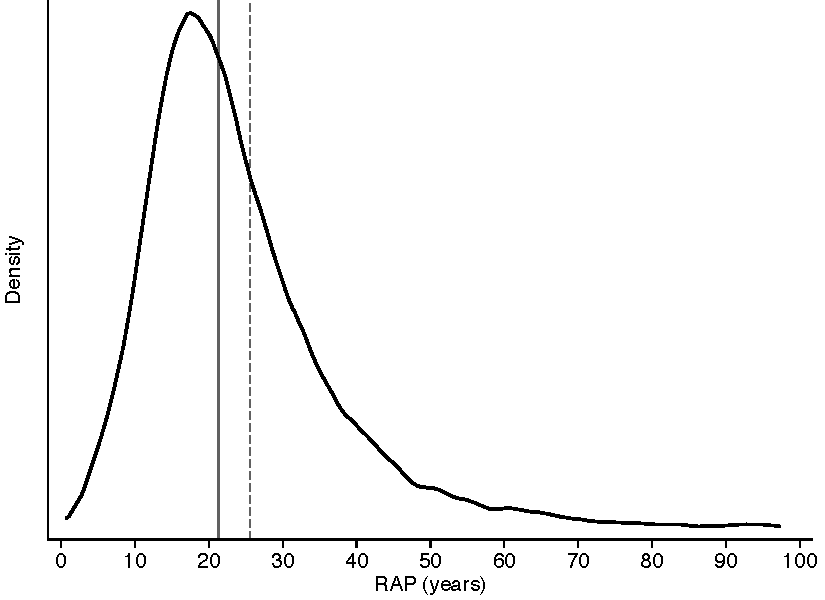
\includegraphics[width=.7\linewidth]{figures/rap_kd.pdf}
\caption[Distribution of biased RAP estimates due to model misspecification in a simulation study]{Distribution of 2,000 RAP estimates from the misspecified logistic model in the simulation study. The dashed vertical line indicates the mean of the distribution (25.4 years), while the solid vertical line indicates the median (21.5 years).}
\label{fig:rap_kd}
\end{figure}

\subsection{Body mass index and prostate cancer mortality rate advancement period}
\label{sec:example_rap_bmi}

Using the updated COSM data presented in section \ref{section:updated_paper1}, we observed no evidence of non-linearity between baseline age and prostate cancer MR ($p_{\textrm{non-linearity}}=0.18$) and, at the same time, the assumption of monotonicity in the age-disease association seemed to hold (data not shown). 

Based on equation (\ref{eq:para_rap}), the RAP comparing obese men at baseline ($\ge 30$ \kgmsq) with normal-weight men (21.0--22.9 \kgmsq) was equal to 18 months. Therefore, under the model, one would expect obese men to experience the same prostate cancer MR as that among normal-weight men who were 18 months older at baseline. The RAP for every 5-unit increment in BMI was equal to 8 months.

Even if there was not enough evidence to reject the linearity assumption in the age-disease relation, the sensitivity of the previous estimates was examined by modeling age with a natural logarithm transform [equation (\ref{eq:para_log_rap}) for RAP applies]. The RAP comparing obese men ($\ge 30$ \kgmsq) with normal-weight men (21.0--22.9 \kgmsq) was equal to 11 months for  men aged 45 years old at baseline and 17 months for  men aged 70 years old. The RAP for every 5-unit increment in BMI increased linearly from 5  to 7 months for men aged 45 and 70 years old, respectively. This, again, illustrates the high sensitivity of RAP to the form of the age-disease dependence.

















